\chapter{SVM e kernel: aspetti pratici e visione critica}\label{ch-14}

Questo pacco di slide completa
\href{13\%20-\%20Support\%20Vector\%20Machines}{13 - Support Vector
Machines} con una visione critica: pregi e difetti delle SVM, esempi di
risultati, il ruolo cruciale degli iperparametri, alcuni luoghi comuni
da sfatare e la generalizzazione ai \textbf{metodi kernel}.

\section{Caratteristiche principali}\label{caratteristiche-principali}

\begin{boxabstract}{Pregi}

\begin{itemize}
\tightlist
\item
  \textbf{Regolarizzazione incorporata} nel problema di ottimizzazione
  (il margine).
\item
  \textbf{Approssimazione della SRM} teorica (il bound sulla VC-dim
  degli iperpiani viene minimizzato dalla soluzione, nel caso hard
  margin senza kernel).
\item
  \textbf{Problema convesso}: l'addestramento trova sempre il
  \textbf{minimo globale} (a differenza delle reti neurali).
\item
  \textbf{Trasformazione implicita delle feature} tramite i kernel.
\end{itemize}

\end{boxabstract}

\begin{boxwarning}{Difetti}

\begin{itemize}
\tightlist
\item
  Bisogna \textbf{scegliere il kernel e i suoi parametri}.
\item
  È un algoritmo \textbf{batch}.
\item
  Problemi molto grandi erano computazionalmente intrattabili: oltre
  circa 20.000 esempi era difficile risolverli esattamente con gli
  approcci standard (la matrice kernel è \(N \times N\)). Oggi esistono
  molte soluzioni, anche basate sulla discesa del gradiente.
\end{itemize}

\end{boxwarning}

In sintesi, i vantaggi:

\begin{itemize}
\tightlist
\item
  un \textbf{modello lineare} (semplice, compatto) con un bound sulla
  complessità in termini di \textbf{margine}, che viene ottimizzato
  direttamente;
\item
  un ricco insieme di \textbf{funzioni di decisione non lineari} nello
  spazio di input tramite i kernel: si fa ancora una separazione
  lineare, ma in uno spazio diverso, con un trattamento
  \textbf{efficiente} della LBE. Un insieme ricco non implica
  necessariamente una VC-dim alta, che per le SVM dipende da margine,
  parametri del kernel, \(C\), ecc.;
\item
  il \textbf{kernel trick} si estende ad altri modelli: i \textbf{metodi
  kernel}.
\end{itemize}

\section{Risultati}\label{risultati}

\subsection{La prima applicazione
famosa}\label{la-prima-applicazione-famosa}

Il riconoscimento di cifre manoscritte (\textbf{MNIST}) fu un caso
storico di successo per le SVM: circa lo 0,8\% di errori nel 1998 con
una SVM polinomiale di grado 9, un risultato notevole, paragonabile a
LeNet e ottenuto senza anni di sviluppo dell'architettura. L'attenzione
per SVM e SLT (i cui studi risalivano agli anni '60--'70) crebbe molto:
un esempio della rilevanza delle applicazioni, o dell'importanza di una
buona teoria per applicazioni di successo.

\subsection{L'esempio della miscela di
gaussiane}\label{lesempio-della-miscela-di-gaussiane}

Riprendiamo il problema delle due classi (miscela di gaussiane) già
visto con i modelli lineari, il K-NN e le reti neurali.

\begin{figure}[htbp]
\centering
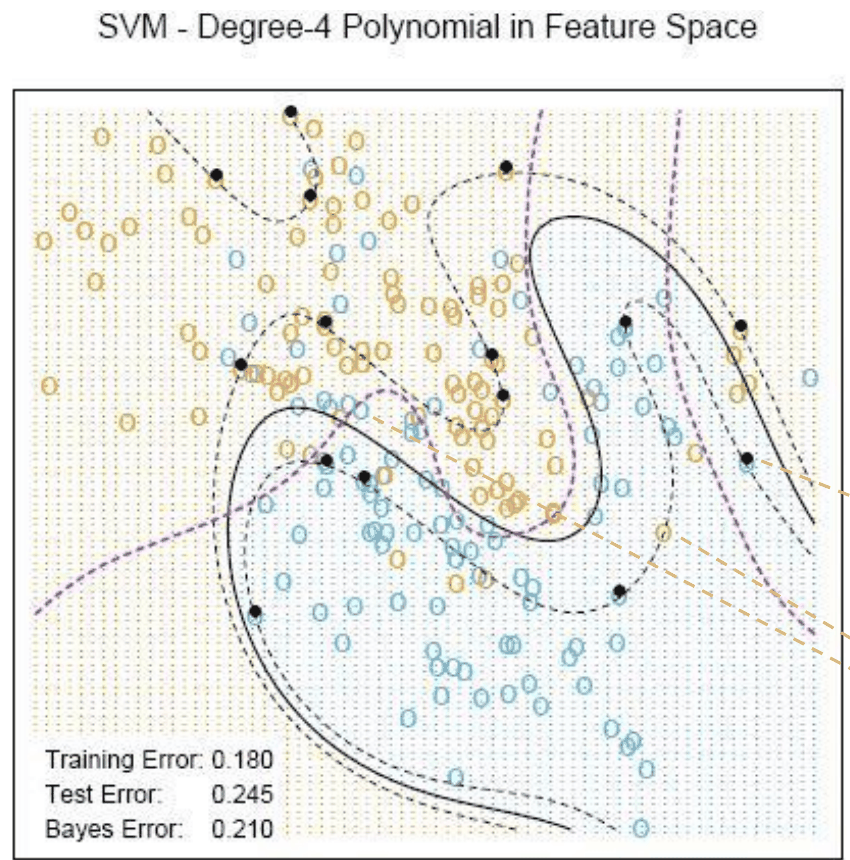
\includegraphics[width=0.51\linewidth,height=0.42\textheight,keepaspectratio]{images/14-svmo_poly.png}
\caption{SVM con kernel polinomiale di grado 4 (\(C = 1\)): il 42\% dei dati
risulta essere support vector.}
\end{figure}

\begin{figure}[htbp]
\centering
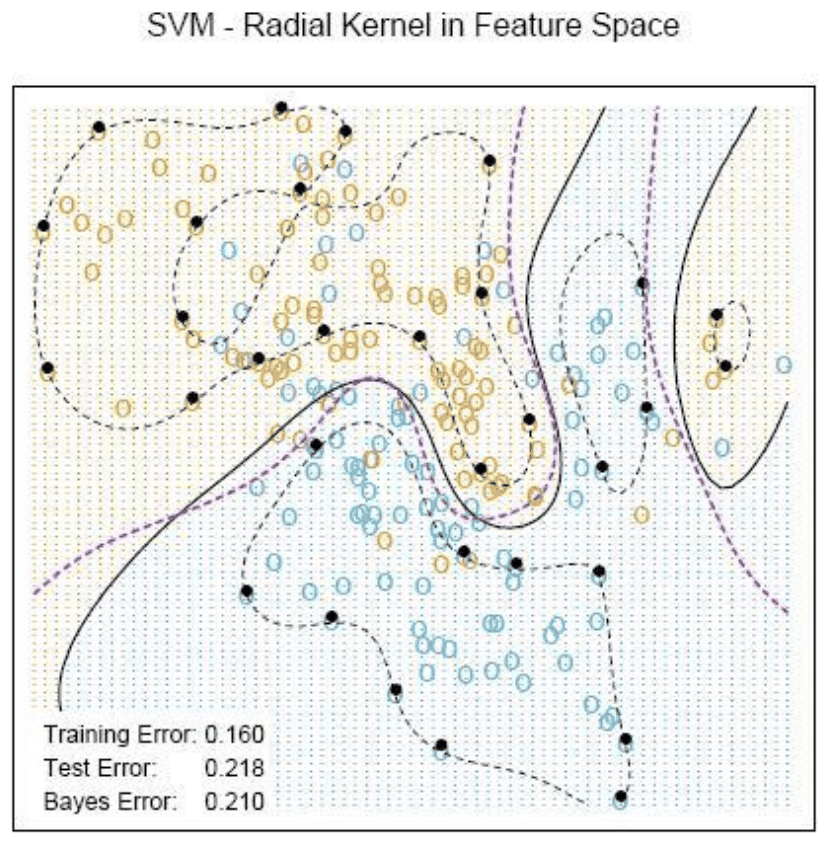
\includegraphics[width=0.51\linewidth,height=0.42\textheight,keepaspectratio]{images/14-svmo_rbf.png}
\caption{SVM con kernel RBF (\(\gamma = 1/(2\sigma^2) = 1\)): il 45\% dei dati
sono support vector.}
\end{figure}

I support vector sono i punti \textbf{sul margine} (slack = 0) o
\textbf{dalla parte sbagliata} del margine (slack \textgreater{} 0). Il
kernel radiale dà il risultato migliore, come ci si può aspettare visto
che i dati provengono da miscele di gaussiane. Si confronti con la rete
neurale con 10 unità e weight decay 0,02 (errore di test 0,223):
risultati simili.

\begin{boxwarning}{Tanti support vector}

Nella teoria si assume che i support vector siano pochi, ma \textbf{non
è sempre vero}: qui sono più del 40\% dei dati. La sparsità della
soluzione non è garantita.

\end{boxwarning}

\section{Le SVM nella pratica}\label{le-svm-nella-pratica}

\begin{boxnote}{Nessuna garanzia}

\emph{``Attualmente non esiste una teoria che garantisca che una data
famiglia di SVM abbia alta accuratezza su un dato problema''} (Burges,
1998).

\end{boxnote}

Le belle proprietà dei classificatori hard margin \textbf{non si
estendono direttamente} al soft margin e ai kernel: il parametro \(C\) e
il kernel possono portare a una VC-dim anche \textbf{infinita}. Ad
esempio:

\begin{itemize}
\tightlist
\item
  una SVM con kernel gaussiano di \textbf{larghezza \(\sigma\)
  sufficientemente piccola} può classificare correttamente un numero
  arbitrariamente grande di punti (come il 1-NN, solo il support vector
  più vicino a \(\mathbf{x}\) contribuisce alla soluzione): VC-dim
  infinita, a meno di regolarizzare;
\item
  all'opposto, con una larghezza \textbf{grande} tutti i support vector
  contribuiscono e si ottiene una sorta di ``media globale'', con VC-dim
  bassa.
\end{itemize}

Quindi \textbf{controllando la larghezza del kernel si controlla la
VC-dim}.

\subsection{Il ruolo critico degli
iperparametri}\label{il-ruolo-critico-degli-iperparametri}

\begin{figure}[htbp]
\centering
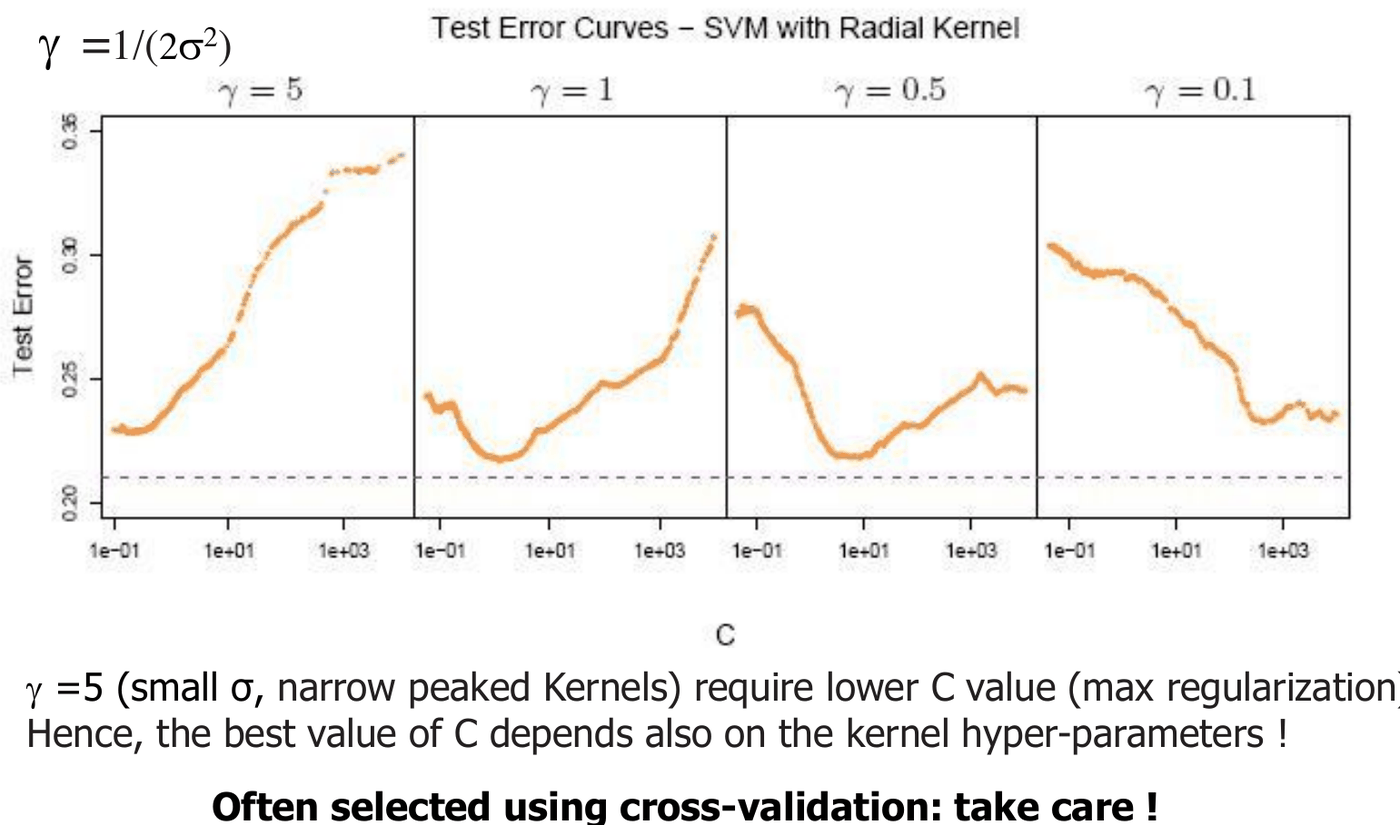
\includegraphics[width=0.86\linewidth,height=0.42\textheight,keepaspectratio]{images/14-svmo_iperparametri.png}
\caption{Errore di test in funzione di \(C\) per diversi valori di
\(\gamma = 1/(2\sigma^2)\).}
\end{figure}

Con \(\gamma = 5\) (piccolo \(\sigma\), kernel molto stretti) serve un
\(C\) basso (massima regolarizzazione); con \(\gamma\) piccoli l'ottimo
si sposta verso \(C\) più alti. \textbf{Il miglior valore di \(C\)
dipende anche dagli iperparametri del kernel}: vanno selezionati
\textbf{insieme} (grid search), di solito con cross-validation, con
attenzione.

Per applicare una SVM bisogna quindi scegliere il \textbf{tipo di
kernel} (e i suoi parametri) e il valore di \textbf{\(C\)} (e di
\(\varepsilon\) per la regressione). Una selezione rigorosa
richiederebbe una stima della complessità (VC-dim); gli iperparametri
che influenzano la complessità sono quelli da usare nella model
selection. In pratica si fa, ancora una volta, una \textbf{valutazione
empirica accurata}: la regolazione degli iperparametri (\(C\),
\(\gamma\)\ldots) può introdurre overfitting, quindi validation set +
test set, oppure double CV.

Prestazioni: spesso buone, ma il confronto con altri metodi non è sempre
favorevole. Dal 2012--2013 le \textbf{reti profonde} hanno superato
nettamente i record precedenti nel riconoscimento di immagini e parlato.

\subsection{Luoghi comuni sulle SVM}\label{luoghi-comuni-sulle-svm}

\begin{boxquestion}{Esercizio: cosa c'è di sbagliato?}

\begin{enumerate}
\def\labelenumi{\arabic{enumi}.}
\tightlist
\item
  \emph{``La SVM si può usare con i valori di default degli
  iperparametri.''} → No: \(C\) e i parametri del kernel sono critici e
  vanno selezionati.
\item
  \emph{``Scelgo la SVM perché non va in overfitting.''} → No: con soft
  margin e kernel la VC-dim può essere altissima; l'overfitting dipende
  da \(C\) e dal kernel.
\item
  \emph{``La SVM non ha problemi con input ad alta dimensione (risolve
  la maledizione della dimensionalità?).''} → \textbf{No}: la SVM
  gestisce bene l'alta dimensione dello \textbf{spazio delle feature},
  non dello \textbf{spazio di input}. La curse of dimensionality
  dell'input resta.
\item
  \emph{``Con la SVM si trova automaticamente il numero di unità.''} →
  Il numero di support vector è determinato dalla soluzione, ma dipende
  da \(C\) e dal kernel, che vanno scelti; e non è detto che sia
  piccolo.
\end{enumerate}

\end{boxquestion}

\section{Metodi kernel}\label{metodi-kernel}

Il \textbf{kernel trick} porta ai \textbf{metodi kernel}, anche senza
SVM: la ``\textbf{kernelizzazione}'' di approcci tradizionali. Ogni
volta che in un modello compare un \textbf{prodotto scalare} o una
\textbf{misura di similarità}, lo si può sostituire con un kernel,
facendo operare il modello in un nuovo spazio implicito ad alta
dimensione semplicemente specificando (e cambiando) il kernel.

\begin{itemize}
\tightlist
\item
  È un'\textbf{espansione lineare in basi} fissa e ad alta dimensione,
  ma molto \textbf{efficiente}.
\item
  La scelta delle funzioni di base è \textbf{modulare}: si cambia il
  kernel senza cambiare la macchina di apprendimento.
\item
  Fornisce un quadro teorico unificato per funzioni generali di tipo
  prodotto scalare.
\end{itemize}

\subsection{Kernel come misura di
similarità}\label{kernel-come-misura-di-similarituxe0}

Il kernel è legato a una misura di \textbf{similarità} tra
\(\mathbf{s}\) e \(\mathbf{t}\); infatti induce la distanza nello spazio
delle feature: \[
d_k(\mathbf{s}, \mathbf{t})^2 = k(\mathbf{s}, \mathbf{s}) - 2k(\mathbf{s}, \mathbf{t}) + k(\mathbf{t}, \mathbf{t}) = \|\Phi(\mathbf{s}) - \Phi(\mathbf{t})\|^2.
\] Oggetti simili (distanza piccola) → valore alto del kernel.

\begin{boxtip}{L'idea dei kernel}

Concentrarsi sulla rappresentazione e l'elaborazione dei
\textbf{confronti tra coppie} di oggetti, anziché sulla rappresentazione
di un singolo oggetto. In alcuni domini è più facile confrontare due
oggetti che definire uno spazio astratto di feature in cui
rappresentarne uno.

\end{boxtip}

Una SVM è caratterizzata in gran parte dalla scelta del kernel. Si
confronti con le \textbf{reti neurali}, dove le funzioni di base si
\textbf{adattano} ai dati (apprendendo i pesi delle unità nascoste):
nelle SVM la scelta del kernel migliore per un problema è ancora un tema
di ricerca.

(Esercizio: ripensare il kernel come nei metodi basati su distanze, tipo
K-NN. Quando un kernel è buono? Quando raggruppa nello spazio delle
feature gli oggetti della stessa classe, riflettendo la similarità
rilevante per il task. Quando è cattivo? Quando la similarità che induce
non ha a che fare con il task, ad esempio se tutti gli oggetti risultano
ugualmente simili o ugualmente diversi.)

\begin{figure}[htbp]
\centering
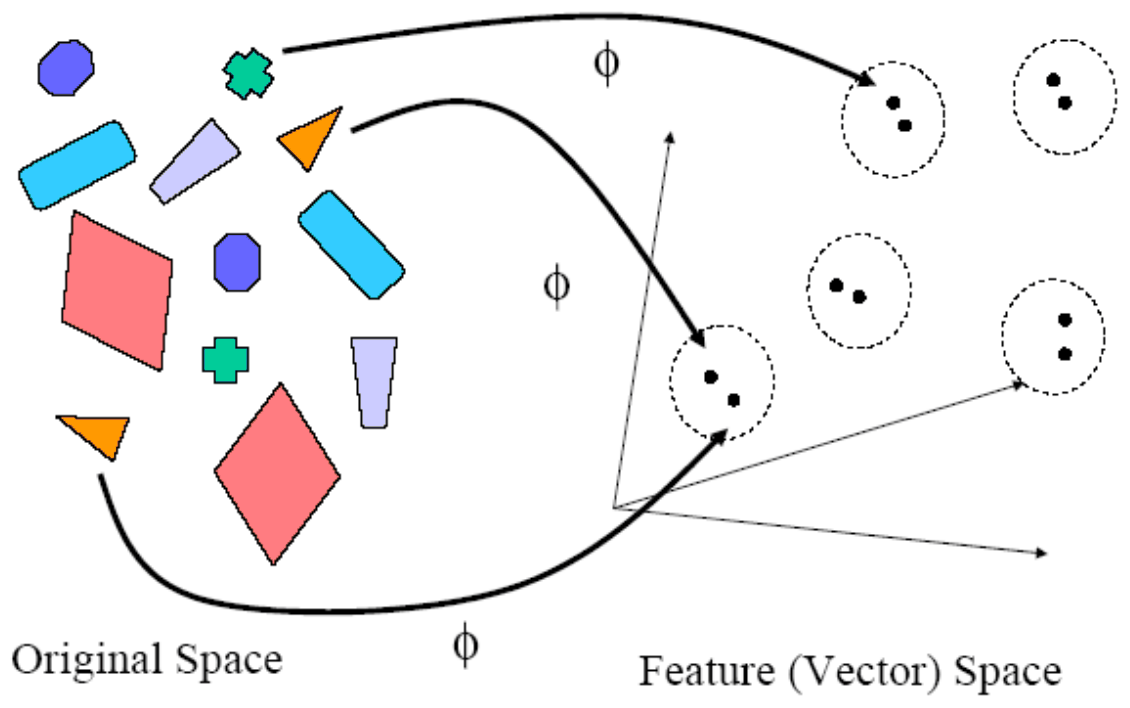
\includegraphics[width=0.63\linewidth,height=0.42\textheight,keepaspectratio]{images/14-svmo_oggetti.png}
\caption{Un buon kernel per ``oggetti'': la mappa \(\phi\) porta oggetti simili
vicini nello spazio delle feature.}
\end{figure}

\subsection{Argomenti avanzati}\label{argomenti-avanzati}

La \textbf{progettazione di nuovi kernel} richiede di scegliere una
funzione ``buona'' per il dominio specifico, e si può estendere a
\textbf{oggetti generici} in input, non solo vettori: kernel per
\textbf{stringhe, alberi, grafi}; kernel ad hoc per il dominio e il task
(ad esempio kernel basati sulla \emph{edit distance} per la
bioinformatica, o su \emph{suffix tree} per stringhe nel NLP), con
attenzione all'efficienza algoritmica. I \textbf{kernel adattivi} sono
un tema di ricerca.

Un vantaggio concettuale: la \textbf{conoscenza di dominio è separata
dal risolutore}, perché sta tutta nel kernel.

\begin{boxabstract}{Sintesi}

Le SVM uniscono un modello lineare, un problema convesso con minimo
globale, la regolarizzazione tramite margine e la potenza dei kernel. Ma
non sono ``magiche'': la scelta di kernel e iperparametri (\(C\),
\(\sigma\), \(\varepsilon\)) è critica e va fatta con una validazione
rigorosa; i support vector possono essere tanti; non risolvono la
maledizione della dimensionalità dello spazio di input. Il kernel trick
è un'idea generale (metodi kernel) che permette di lavorare con
similarità tra oggetti anche strutturati.

\end{boxabstract}

\begin{boxquestion}{Possibili domande d'esame}

\begin{itemize}
\tightlist
\item
  Pregi e difetti delle SVM rispetto alle reti neurali.
\item
  Perché la VC-dim di una SVM con kernel RBF può essere infinita? Come
  si controlla?
\item
  Perché \(C\) e i parametri del kernel vanno selezionati insieme?
\item
  La SVM risolve la maledizione della dimensionalità?
\item
  Cosa sono i metodi kernel? Che legame c'è tra kernel e similarità?
\end{itemize}

\end{boxquestion}
